%----------------------------------------------------------------
\begin{frame}[fragile]{Unitary tests cases}

\begin{itemize}
    \item Check \cred{regression}  of the code to previous state
    \item Some of them acts as \cred{validation} tests cases
    \item Intended also for \cred{future handbook/tutorials}

\begin{center}
\begin{minipage}{0.45\textwidth}
        \begin{itemize}
            \item Test incidence matrix
            \item Test basic geometry computations
            \item Test on ADP, R, $\Phi$ matrices
            \item Test assembled system
            \item Test Linearized fluid-dynamic solver
        \end{itemize}
\end{minipage}%
\hfill
\begin{minipage}{0.45\textwidth}
\begin{minted}[linenos=true,numbersep=1pt,frame=lines,framesep=2mm,fontsize=\tiny, bgcolor=background]{cpp}
int main(int argc, char **argv)
{
    using triple_t = std::array<double, 3>;
    using sparse_matrix_t = Eigen::SparseMatrix<double>; 
    
    infrastructure_graph igraph;
    make_init_graph(igraph);

    incidence inc(igraph);
    const sparse_matrix_t& mat  = inc.matrix();

    std::cout << __FILE__ << std::endl;
    bool pass = verify_test("incidence matrix", mat, ref);
    
    return !pass; 
}
\end{minted}    
\end{minipage}%    
\end{center}
\end{itemize}
\end{frame}
%----------------------------------------------------------------
\begin{frame}{What shimmer++ does not}

\begin{itemize}

    \item Does \cred{not transform units}. So input data must be given in \dgreen{SI units}
    \item Non-pipe elements (yet)
    \begin{figure}
        \centering
    \includegraphics[scale = 0.5]{img_other/non_pipe_elements.png}
    \end{figure}
    \item No refinement per pipe (grid creator)
    \begin{center}    % Graphic for TeX using PGF
% Title: /home/karol/Documents/UNIVERSITA/POLITO/PRESENTATIONS/SHIMMER_2024_01/img_code/pipe_network_ref.dia
% Creator: Dia v0.97.3
% CreationDate: Tue Jan 30 23:44:31 2024
% For: karol
% \usepackage{tikz}
% The following commands are not supported in PSTricks at present
% We define them conditionally, so when they are implemented,
% this pgf file will use them.
\ifx\du\undefined
  \newlength{\du}
\fi
\setlength{\du}{8\unitlength}
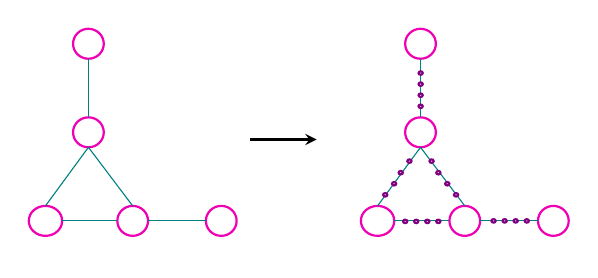
\begin{tikzpicture}[even odd rule]
\pgftransformxscale{1.000000}
\pgftransformyscale{-1.000000}
\definecolor{dialinecolor}{rgb}{0.000000, 0.000000, 0.000000}
\pgfsetstrokecolor{dialinecolor}
\pgfsetstrokeopacity{1.000000}
\definecolor{diafillcolor}{rgb}{1.000000, 1.000000, 1.000000}
\pgfsetfillcolor{diafillcolor}
\pgfsetfillopacity{1.000000}
\pgfsetlinewidth{0.100000\du}
\pgfsetdash{}{0pt}
\pgfsetmiterjoin
\definecolor{diafillcolor}{rgb}{1.000000, 1.000000, 1.000000}
\pgfsetfillcolor{diafillcolor}
\pgfsetfillopacity{1.000000}
\pgfpathellipse{\pgfpoint{39.693572\du}{5.676288\du}}{\pgfpoint{0.693572\du}{0\du}}{\pgfpoint{0\du}{0.676288\du}}
\pgfusepath{fill}
\definecolor{dialinecolor}{rgb}{0.937255, 0.000000, 0.701961}
\pgfsetstrokecolor{dialinecolor}
\pgfsetstrokeopacity{1.000000}
\pgfpathellipse{\pgfpoint{39.693572\du}{5.676288\du}}{\pgfpoint{0.693572\du}{0\du}}{\pgfpoint{0\du}{0.676288\du}}
\pgfusepath{stroke}
% setfont left to latex
% setfont left to latex
\definecolor{dialinecolor}{rgb}{0.000000, 0.000000, 0.000000}
\pgfsetstrokecolor{dialinecolor}
\pgfsetstrokeopacity{1.000000}
\definecolor{diafillcolor}{rgb}{0.000000, 0.000000, 0.000000}
\pgfsetfillcolor{diafillcolor}
\pgfsetfillopacity{1.000000}
\node[anchor=base,inner sep=0pt, outer sep=0pt,color=dialinecolor] at (39.693572\du,5.961288\du){};
\pgfsetlinewidth{0.100000\du}
\pgfsetdash{}{0pt}
\pgfsetmiterjoin
\definecolor{diafillcolor}{rgb}{1.000000, 1.000000, 1.000000}
\pgfsetfillcolor{diafillcolor}
\pgfsetfillopacity{1.000000}
\pgfpathellipse{\pgfpoint{39.693572\du}{9.676288\du}}{\pgfpoint{0.693572\du}{0\du}}{\pgfpoint{0\du}{0.676288\du}}
\pgfusepath{fill}
\definecolor{dialinecolor}{rgb}{0.937255, 0.000000, 0.701961}
\pgfsetstrokecolor{dialinecolor}
\pgfsetstrokeopacity{1.000000}
\pgfpathellipse{\pgfpoint{39.693572\du}{9.676288\du}}{\pgfpoint{0.693572\du}{0\du}}{\pgfpoint{0\du}{0.676288\du}}
\pgfusepath{stroke}
% setfont left to latex
% setfont left to latex
\definecolor{dialinecolor}{rgb}{0.000000, 0.000000, 0.000000}
\pgfsetstrokecolor{dialinecolor}
\pgfsetstrokeopacity{1.000000}
\definecolor{diafillcolor}{rgb}{0.000000, 0.000000, 0.000000}
\pgfsetfillcolor{diafillcolor}
\pgfsetfillopacity{1.000000}
\node[anchor=base,inner sep=0pt, outer sep=0pt,color=dialinecolor] at (39.693572\du,9.961288\du){};
\pgfsetlinewidth{0.100000\du}
\pgfsetdash{}{0pt}
\pgfsetmiterjoin
\definecolor{diafillcolor}{rgb}{1.000000, 1.000000, 1.000000}
\pgfsetfillcolor{diafillcolor}
\pgfsetfillopacity{1.000000}
\pgfpathellipse{\pgfpoint{37.753572\du}{13.676288\du}}{\pgfpoint{0.753572\du}{0\du}}{\pgfpoint{0\du}{0.676288\du}}
\pgfusepath{fill}
\definecolor{dialinecolor}{rgb}{0.937255, 0.000000, 0.701961}
\pgfsetstrokecolor{dialinecolor}
\pgfsetstrokeopacity{1.000000}
\pgfpathellipse{\pgfpoint{37.753572\du}{13.676288\du}}{\pgfpoint{0.753572\du}{0\du}}{\pgfpoint{0\du}{0.676288\du}}
\pgfusepath{stroke}
% setfont left to latex
% setfont left to latex
\definecolor{dialinecolor}{rgb}{0.000000, 0.000000, 0.000000}
\pgfsetstrokecolor{dialinecolor}
\pgfsetstrokeopacity{1.000000}
\definecolor{diafillcolor}{rgb}{0.000000, 0.000000, 0.000000}
\pgfsetfillcolor{diafillcolor}
\pgfsetfillopacity{1.000000}
\node[anchor=base,inner sep=0pt, outer sep=0pt,color=dialinecolor] at (37.753572\du,13.961288\du){};
\pgfsetlinewidth{0.100000\du}
\pgfsetdash{}{0pt}
\pgfsetmiterjoin
\definecolor{diafillcolor}{rgb}{1.000000, 1.000000, 1.000000}
\pgfsetfillcolor{diafillcolor}
\pgfsetfillopacity{1.000000}
\pgfpathellipse{\pgfpoint{45.693572\du}{13.676288\du}}{\pgfpoint{0.693572\du}{0\du}}{\pgfpoint{0\du}{0.676288\du}}
\pgfusepath{fill}
\definecolor{dialinecolor}{rgb}{0.937255, 0.000000, 0.701961}
\pgfsetstrokecolor{dialinecolor}
\pgfsetstrokeopacity{1.000000}
\pgfpathellipse{\pgfpoint{45.693572\du}{13.676288\du}}{\pgfpoint{0.693572\du}{0\du}}{\pgfpoint{0\du}{0.676288\du}}
\pgfusepath{stroke}
% setfont left to latex
% setfont left to latex
\definecolor{dialinecolor}{rgb}{0.000000, 0.000000, 0.000000}
\pgfsetstrokecolor{dialinecolor}
\pgfsetstrokeopacity{1.000000}
\definecolor{diafillcolor}{rgb}{0.000000, 0.000000, 0.000000}
\pgfsetfillcolor{diafillcolor}
\pgfsetfillopacity{1.000000}
\node[anchor=base,inner sep=0pt, outer sep=0pt,color=dialinecolor] at (45.693572\du,13.961288\du){};
\pgfsetlinewidth{0.100000\du}
\pgfsetdash{}{0pt}
\pgfsetmiterjoin
\definecolor{diafillcolor}{rgb}{1.000000, 1.000000, 1.000000}
\pgfsetfillcolor{diafillcolor}
\pgfsetfillopacity{1.000000}
\pgfpathellipse{\pgfpoint{41.693572\du}{13.676288\du}}{\pgfpoint{0.693572\du}{0\du}}{\pgfpoint{0\du}{0.676288\du}}
\pgfusepath{fill}
\definecolor{dialinecolor}{rgb}{0.937255, 0.000000, 0.701961}
\pgfsetstrokecolor{dialinecolor}
\pgfsetstrokeopacity{1.000000}
\pgfpathellipse{\pgfpoint{41.693572\du}{13.676288\du}}{\pgfpoint{0.693572\du}{0\du}}{\pgfpoint{0\du}{0.676288\du}}
\pgfusepath{stroke}
% setfont left to latex
% setfont left to latex
\definecolor{dialinecolor}{rgb}{0.000000, 0.000000, 0.000000}
\pgfsetstrokecolor{dialinecolor}
\pgfsetstrokeopacity{1.000000}
\definecolor{diafillcolor}{rgb}{0.000000, 0.000000, 0.000000}
\pgfsetfillcolor{diafillcolor}
\pgfsetfillopacity{1.000000}
\node[anchor=base,inner sep=0pt, outer sep=0pt,color=dialinecolor] at (41.693572\du,13.961288\du){};
\pgfsetlinewidth{0.050000\du}
\pgfsetdash{}{0pt}
\pgfsetbuttcap
{
\definecolor{diafillcolor}{rgb}{0.000000, 0.501961, 0.501961}
\pgfsetfillcolor{diafillcolor}
\pgfsetfillopacity{1.000000}
% was here!!!
\definecolor{dialinecolor}{rgb}{0.000000, 0.501961, 0.501961}
\pgfsetstrokecolor{dialinecolor}
\pgfsetstrokeopacity{1.000000}
\draw (39.693572\du,6.351417\du)--(39.693570\du,9.000000\du);
}
\pgfsetlinewidth{0.050000\du}
\pgfsetdash{}{0pt}
\pgfsetbuttcap
{
\definecolor{diafillcolor}{rgb}{0.000000, 0.501961, 0.501961}
\pgfsetfillcolor{diafillcolor}
\pgfsetfillopacity{1.000000}
% was here!!!
\definecolor{dialinecolor}{rgb}{0.000000, 0.501961, 0.501961}
\pgfsetstrokecolor{dialinecolor}
\pgfsetstrokeopacity{1.000000}
\draw (39.693570\du,10.352600\du)--(37.753570\du,13.000000\du);
}
\pgfsetlinewidth{0.050000\du}
\pgfsetdash{}{0pt}
\pgfsetbuttcap
{
\definecolor{diafillcolor}{rgb}{0.000000, 0.501961, 0.501961}
\pgfsetfillcolor{diafillcolor}
\pgfsetfillopacity{1.000000}
% was here!!!
\definecolor{dialinecolor}{rgb}{0.000000, 0.501961, 0.501961}
\pgfsetstrokecolor{dialinecolor}
\pgfsetstrokeopacity{1.000000}
\draw (39.693570\du,10.352600\du)--(41.693600\du,13.000000\du);
}
\pgfsetlinewidth{0.050000\du}
\pgfsetdash{}{0pt}
\pgfsetbuttcap
{
\definecolor{diafillcolor}{rgb}{0.000000, 0.501961, 0.501961}
\pgfsetfillcolor{diafillcolor}
\pgfsetfillopacity{1.000000}
% was here!!!
\definecolor{dialinecolor}{rgb}{0.000000, 0.501961, 0.501961}
\pgfsetstrokecolor{dialinecolor}
\pgfsetstrokeopacity{1.000000}
\draw (41.000000\du,13.676300\du)--(38.507140\du,13.676300\du);
}
\pgfsetlinewidth{0.050000\du}
\pgfsetdash{}{0pt}
\pgfsetbuttcap
{
\definecolor{diafillcolor}{rgb}{0.000000, 0.501961, 0.501961}
\pgfsetfillcolor{diafillcolor}
\pgfsetfillopacity{1.000000}
% was here!!!
\definecolor{dialinecolor}{rgb}{0.000000, 0.501961, 0.501961}
\pgfsetstrokecolor{dialinecolor}
\pgfsetstrokeopacity{1.000000}
\draw (42.387100\du,13.676300\du)--(45.000000\du,13.676300\du);
}
% setfont left to latex
% setfont left to latex
\definecolor{dialinecolor}{rgb}{0.000000, 0.501961, 0.501961}
\pgfsetstrokecolor{dialinecolor}
\pgfsetstrokeopacity{1.000000}
\definecolor{diafillcolor}{rgb}{0.000000, 0.501961, 0.501961}
\pgfsetfillcolor{diafillcolor}
\pgfsetfillopacity{1.000000}
\node[anchor=base west,inner sep=0pt,outer sep=0pt,color=dialinecolor] at (39.000000\du,8.000000\du){};
% setfont left to latex
% setfont left to latex
\definecolor{dialinecolor}{rgb}{0.000000, 0.501961, 0.501961}
\pgfsetstrokecolor{dialinecolor}
\pgfsetstrokeopacity{1.000000}
\definecolor{diafillcolor}{rgb}{0.000000, 0.501961, 0.501961}
\pgfsetfillcolor{diafillcolor}
\pgfsetfillopacity{1.000000}
\node[anchor=base west,inner sep=0pt,outer sep=0pt,color=dialinecolor] at (38.000000\du,12.000000\du){};
% setfont left to latex
% setfont left to latex
\definecolor{dialinecolor}{rgb}{0.000000, 0.501961, 0.501961}
\pgfsetstrokecolor{dialinecolor}
\pgfsetstrokeopacity{1.000000}
\definecolor{diafillcolor}{rgb}{0.000000, 0.501961, 0.501961}
\pgfsetfillcolor{diafillcolor}
\pgfsetfillopacity{1.000000}
\node[anchor=base west,inner sep=0pt,outer sep=0pt,color=dialinecolor] at (42.000000\du,12.000000\du){};
% setfont left to latex
% setfont left to latex
\definecolor{dialinecolor}{rgb}{0.000000, 0.501961, 0.501961}
\pgfsetstrokecolor{dialinecolor}
\pgfsetstrokeopacity{1.000000}
\definecolor{diafillcolor}{rgb}{0.000000, 0.501961, 0.501961}
\pgfsetfillcolor{diafillcolor}
\pgfsetfillopacity{1.000000}
\node[anchor=base west,inner sep=0pt,outer sep=0pt,color=dialinecolor] at (39.450000\du,14.900000\du){};
% setfont left to latex
% setfont left to latex
\definecolor{dialinecolor}{rgb}{0.000000, 0.501961, 0.501961}
\pgfsetstrokecolor{dialinecolor}
\pgfsetstrokeopacity{1.000000}
\definecolor{diafillcolor}{rgb}{0.000000, 0.501961, 0.501961}
\pgfsetfillcolor{diafillcolor}
\pgfsetfillopacity{1.000000}
\node[anchor=base west,inner sep=0pt,outer sep=0pt,color=dialinecolor] at (43.590000\du,14.895000\du){};
\pgfsetlinewidth{0.100000\du}
\pgfsetdash{}{0pt}
\definecolor{diafillcolor}{rgb}{1.000000, 1.000000, 1.000000}
\pgfsetfillcolor{diafillcolor}
\pgfsetfillopacity{1.000000}
\pgfpathellipse{\pgfpoint{39.700000\du}{7.499999\du}}{\pgfpoint{0.093210\du}{0\du}}{\pgfpoint{0\du}{0.076999\du}}
\pgfusepath{fill}
\definecolor{dialinecolor}{rgb}{0.501961, 0.000000, 0.501961}
\pgfsetstrokecolor{dialinecolor}
\pgfsetstrokeopacity{1.000000}
\pgfpathellipse{\pgfpoint{39.700000\du}{7.499999\du}}{\pgfpoint{0.093210\du}{0\du}}{\pgfpoint{0\du}{0.076999\du}}
\pgfusepath{stroke}
\pgfsetlinewidth{0.100000\du}
\pgfsetdash{}{0pt}
\definecolor{diafillcolor}{rgb}{1.000000, 1.000000, 1.000000}
\pgfsetfillcolor{diafillcolor}
\pgfsetfillopacity{1.000000}
\pgfpathellipse{\pgfpoint{39.700000\du}{6.999999\du}}{\pgfpoint{0.093210\du}{0\du}}{\pgfpoint{0\du}{0.076999\du}}
\pgfusepath{fill}
\definecolor{dialinecolor}{rgb}{0.501961, 0.000000, 0.501961}
\pgfsetstrokecolor{dialinecolor}
\pgfsetstrokeopacity{1.000000}
\pgfpathellipse{\pgfpoint{39.700000\du}{6.999999\du}}{\pgfpoint{0.093210\du}{0\du}}{\pgfpoint{0\du}{0.076999\du}}
\pgfusepath{stroke}
\pgfsetlinewidth{0.100000\du}
\pgfsetdash{}{0pt}
\definecolor{diafillcolor}{rgb}{1.000000, 1.000000, 1.000000}
\pgfsetfillcolor{diafillcolor}
\pgfsetfillopacity{1.000000}
\pgfpathellipse{\pgfpoint{39.700000\du}{7.999999\du}}{\pgfpoint{0.093210\du}{0\du}}{\pgfpoint{0\du}{0.076999\du}}
\pgfusepath{fill}
\definecolor{dialinecolor}{rgb}{0.501961, 0.000000, 0.501961}
\pgfsetstrokecolor{dialinecolor}
\pgfsetstrokeopacity{1.000000}
\pgfpathellipse{\pgfpoint{39.700000\du}{7.999999\du}}{\pgfpoint{0.093210\du}{0\du}}{\pgfpoint{0\du}{0.076999\du}}
\pgfusepath{stroke}
\pgfsetlinewidth{0.100000\du}
\pgfsetdash{}{0pt}
\definecolor{diafillcolor}{rgb}{1.000000, 1.000000, 1.000000}
\pgfsetfillcolor{diafillcolor}
\pgfsetfillopacity{1.000000}
\pgfpathellipse{\pgfpoint{39.700000\du}{8.499999\du}}{\pgfpoint{0.093210\du}{0\du}}{\pgfpoint{0\du}{0.076999\du}}
\pgfusepath{fill}
\definecolor{dialinecolor}{rgb}{0.501961, 0.000000, 0.501961}
\pgfsetstrokecolor{dialinecolor}
\pgfsetstrokeopacity{1.000000}
\pgfpathellipse{\pgfpoint{39.700000\du}{8.499999\du}}{\pgfpoint{0.093210\du}{0\du}}{\pgfpoint{0\du}{0.076999\du}}
\pgfusepath{stroke}
\pgfsetlinewidth{0.100000\du}
\pgfsetdash{}{0pt}
\definecolor{diafillcolor}{rgb}{1.000000, 1.000000, 1.000000}
\pgfsetfillcolor{diafillcolor}
\pgfsetfillopacity{1.000000}
\pgfpathellipse{\pgfpoint{40.500000\du}{11.499999\du}}{\pgfpoint{0.093210\du}{0\du}}{\pgfpoint{0\du}{0.076999\du}}
\pgfusepath{fill}
\definecolor{dialinecolor}{rgb}{0.501961, 0.000000, 0.501961}
\pgfsetstrokecolor{dialinecolor}
\pgfsetstrokeopacity{1.000000}
\pgfpathellipse{\pgfpoint{40.500000\du}{11.499999\du}}{\pgfpoint{0.093210\du}{0\du}}{\pgfpoint{0\du}{0.076999\du}}
\pgfusepath{stroke}
\pgfsetlinewidth{0.100000\du}
\pgfsetdash{}{0pt}
\definecolor{diafillcolor}{rgb}{1.000000, 1.000000, 1.000000}
\pgfsetfillcolor{diafillcolor}
\pgfsetfillopacity{1.000000}
\pgfpathellipse{\pgfpoint{40.193210\du}{10.976999\du}}{\pgfpoint{0.093210\du}{0\du}}{\pgfpoint{0\du}{0.076999\du}}
\pgfusepath{fill}
\definecolor{dialinecolor}{rgb}{0.501961, 0.000000, 0.501961}
\pgfsetstrokecolor{dialinecolor}
\pgfsetstrokeopacity{1.000000}
\pgfpathellipse{\pgfpoint{40.193210\du}{10.976999\du}}{\pgfpoint{0.093210\du}{0\du}}{\pgfpoint{0\du}{0.076999\du}}
\pgfusepath{stroke}
\pgfsetlinewidth{0.100000\du}
\pgfsetdash{}{0pt}
\definecolor{diafillcolor}{rgb}{1.000000, 1.000000, 1.000000}
\pgfsetfillcolor{diafillcolor}
\pgfsetfillopacity{1.000000}
\pgfpathellipse{\pgfpoint{40.900000\du}{11.999999\du}}{\pgfpoint{0.093210\du}{0\du}}{\pgfpoint{0\du}{0.076999\du}}
\pgfusepath{fill}
\definecolor{dialinecolor}{rgb}{0.501961, 0.000000, 0.501961}
\pgfsetstrokecolor{dialinecolor}
\pgfsetstrokeopacity{1.000000}
\pgfpathellipse{\pgfpoint{40.900000\du}{11.999999\du}}{\pgfpoint{0.093210\du}{0\du}}{\pgfpoint{0\du}{0.076999\du}}
\pgfusepath{stroke}
\pgfsetlinewidth{0.100000\du}
\pgfsetdash{}{0pt}
\definecolor{diafillcolor}{rgb}{1.000000, 1.000000, 1.000000}
\pgfsetfillcolor{diafillcolor}
\pgfsetfillopacity{1.000000}
\pgfpathellipse{\pgfpoint{41.300010\du}{12.499999\du}}{\pgfpoint{0.093210\du}{0\du}}{\pgfpoint{0\du}{0.076999\du}}
\pgfusepath{fill}
\definecolor{dialinecolor}{rgb}{0.501961, 0.000000, 0.501961}
\pgfsetstrokecolor{dialinecolor}
\pgfsetstrokeopacity{1.000000}
\pgfpathellipse{\pgfpoint{41.300010\du}{12.499999\du}}{\pgfpoint{0.093210\du}{0\du}}{\pgfpoint{0\du}{0.076999\du}}
\pgfusepath{stroke}
\pgfsetlinewidth{0.100000\du}
\pgfsetdash{}{0pt}
\definecolor{diafillcolor}{rgb}{1.000000, 1.000000, 1.000000}
\pgfsetfillcolor{diafillcolor}
\pgfsetfillopacity{1.000000}
\pgfpathellipse{\pgfpoint{38.800000\du}{11.499999\du}}{\pgfpoint{0.093210\du}{0\du}}{\pgfpoint{0\du}{0.076999\du}}
\pgfusepath{fill}
\definecolor{dialinecolor}{rgb}{0.501961, 0.000000, 0.501961}
\pgfsetstrokecolor{dialinecolor}
\pgfsetstrokeopacity{1.000000}
\pgfpathellipse{\pgfpoint{38.800000\du}{11.499999\du}}{\pgfpoint{0.093210\du}{0\du}}{\pgfpoint{0\du}{0.076999\du}}
\pgfusepath{stroke}
\pgfsetlinewidth{0.100000\du}
\pgfsetdash{}{0pt}
\definecolor{diafillcolor}{rgb}{1.000000, 1.000000, 1.000000}
\pgfsetfillcolor{diafillcolor}
\pgfsetfillopacity{1.000000}
\pgfpathellipse{\pgfpoint{39.193210\du}{10.976999\du}}{\pgfpoint{0.093210\du}{0\du}}{\pgfpoint{0\du}{0.076999\du}}
\pgfusepath{fill}
\definecolor{dialinecolor}{rgb}{0.501961, 0.000000, 0.501961}
\pgfsetstrokecolor{dialinecolor}
\pgfsetstrokeopacity{1.000000}
\pgfpathellipse{\pgfpoint{39.193210\du}{10.976999\du}}{\pgfpoint{0.093210\du}{0\du}}{\pgfpoint{0\du}{0.076999\du}}
\pgfusepath{stroke}
\pgfsetlinewidth{0.100000\du}
\pgfsetdash{}{0pt}
\definecolor{diafillcolor}{rgb}{1.000000, 1.000000, 1.000000}
\pgfsetfillcolor{diafillcolor}
\pgfsetfillopacity{1.000000}
\pgfpathellipse{\pgfpoint{38.500000\du}{11.999999\du}}{\pgfpoint{0.093210\du}{0\du}}{\pgfpoint{0\du}{0.076999\du}}
\pgfusepath{fill}
\definecolor{dialinecolor}{rgb}{0.501961, 0.000000, 0.501961}
\pgfsetstrokecolor{dialinecolor}
\pgfsetstrokeopacity{1.000000}
\pgfpathellipse{\pgfpoint{38.500000\du}{11.999999\du}}{\pgfpoint{0.093210\du}{0\du}}{\pgfpoint{0\du}{0.076999\du}}
\pgfusepath{stroke}
\pgfsetlinewidth{0.100000\du}
\pgfsetdash{}{0pt}
\definecolor{diafillcolor}{rgb}{1.000000, 1.000000, 1.000000}
\pgfsetfillcolor{diafillcolor}
\pgfsetfillopacity{1.000000}
\pgfpathellipse{\pgfpoint{38.100000\du}{12.499999\du}}{\pgfpoint{0.093210\du}{0\du}}{\pgfpoint{0\du}{0.076999\du}}
\pgfusepath{fill}
\definecolor{dialinecolor}{rgb}{0.501961, 0.000000, 0.501961}
\pgfsetstrokecolor{dialinecolor}
\pgfsetstrokeopacity{1.000000}
\pgfpathellipse{\pgfpoint{38.100000\du}{12.499999\du}}{\pgfpoint{0.093210\du}{0\du}}{\pgfpoint{0\du}{0.076999\du}}
\pgfusepath{stroke}
\pgfsetlinewidth{0.100000\du}
\pgfsetdash{}{0pt}
\definecolor{diafillcolor}{rgb}{1.000000, 1.000000, 1.000000}
\pgfsetfillcolor{diafillcolor}
\pgfsetfillopacity{1.000000}
\pgfpathellipse{\pgfpoint{39.500000\du}{13.699999\du}}{\pgfpoint{0.093210\du}{0\du}}{\pgfpoint{0\du}{0.076999\du}}
\pgfusepath{fill}
\definecolor{dialinecolor}{rgb}{0.501961, 0.000000, 0.501961}
\pgfsetstrokecolor{dialinecolor}
\pgfsetstrokeopacity{1.000000}
\pgfpathellipse{\pgfpoint{39.500000\du}{13.699999\du}}{\pgfpoint{0.093210\du}{0\du}}{\pgfpoint{0\du}{0.076999\du}}
\pgfusepath{stroke}
\pgfsetlinewidth{0.100000\du}
\pgfsetdash{}{0pt}
\definecolor{diafillcolor}{rgb}{1.000000, 1.000000, 1.000000}
\pgfsetfillcolor{diafillcolor}
\pgfsetfillopacity{1.000000}
\pgfpathellipse{\pgfpoint{39.000000\du}{13.699999\du}}{\pgfpoint{0.093210\du}{0\du}}{\pgfpoint{0\du}{0.076999\du}}
\pgfusepath{fill}
\definecolor{dialinecolor}{rgb}{0.501961, 0.000000, 0.501961}
\pgfsetstrokecolor{dialinecolor}
\pgfsetstrokeopacity{1.000000}
\pgfpathellipse{\pgfpoint{39.000000\du}{13.699999\du}}{\pgfpoint{0.093210\du}{0\du}}{\pgfpoint{0\du}{0.076999\du}}
\pgfusepath{stroke}
\pgfsetlinewidth{0.100000\du}
\pgfsetdash{}{0pt}
\definecolor{diafillcolor}{rgb}{1.000000, 1.000000, 1.000000}
\pgfsetfillcolor{diafillcolor}
\pgfsetfillopacity{1.000000}
\pgfpathellipse{\pgfpoint{40.000000\du}{13.699999\du}}{\pgfpoint{0.093210\du}{0\du}}{\pgfpoint{0\du}{0.076999\du}}
\pgfusepath{fill}
\definecolor{dialinecolor}{rgb}{0.501961, 0.000000, 0.501961}
\pgfsetstrokecolor{dialinecolor}
\pgfsetstrokeopacity{1.000000}
\pgfpathellipse{\pgfpoint{40.000000\du}{13.699999\du}}{\pgfpoint{0.093210\du}{0\du}}{\pgfpoint{0\du}{0.076999\du}}
\pgfusepath{stroke}
\pgfsetlinewidth{0.100000\du}
\pgfsetdash{}{0pt}
\definecolor{diafillcolor}{rgb}{1.000000, 1.000000, 1.000000}
\pgfsetfillcolor{diafillcolor}
\pgfsetfillopacity{1.000000}
\pgfpathellipse{\pgfpoint{40.500000\du}{13.699999\du}}{\pgfpoint{0.093210\du}{0\du}}{\pgfpoint{0\du}{0.076999\du}}
\pgfusepath{fill}
\definecolor{dialinecolor}{rgb}{0.501961, 0.000000, 0.501961}
\pgfsetstrokecolor{dialinecolor}
\pgfsetstrokeopacity{1.000000}
\pgfpathellipse{\pgfpoint{40.500000\du}{13.699999\du}}{\pgfpoint{0.093210\du}{0\du}}{\pgfpoint{0\du}{0.076999\du}}
\pgfusepath{stroke}
\pgfsetlinewidth{0.100000\du}
\pgfsetdash{}{0pt}
\definecolor{diafillcolor}{rgb}{1.000000, 1.000000, 1.000000}
\pgfsetfillcolor{diafillcolor}
\pgfsetfillopacity{1.000000}
\pgfpathellipse{\pgfpoint{43.493210\du}{13.676999\du}}{\pgfpoint{0.093210\du}{0\du}}{\pgfpoint{0\du}{0.076999\du}}
\pgfusepath{fill}
\definecolor{dialinecolor}{rgb}{0.501961, 0.000000, 0.501961}
\pgfsetstrokecolor{dialinecolor}
\pgfsetstrokeopacity{1.000000}
\pgfpathellipse{\pgfpoint{43.493210\du}{13.676999\du}}{\pgfpoint{0.093210\du}{0\du}}{\pgfpoint{0\du}{0.076999\du}}
\pgfusepath{stroke}
\pgfsetlinewidth{0.100000\du}
\pgfsetdash{}{0pt}
\definecolor{diafillcolor}{rgb}{1.000000, 1.000000, 1.000000}
\pgfsetfillcolor{diafillcolor}
\pgfsetfillopacity{1.000000}
\pgfpathellipse{\pgfpoint{42.993210\du}{13.676999\du}}{\pgfpoint{0.093210\du}{0\du}}{\pgfpoint{0\du}{0.076999\du}}
\pgfusepath{fill}
\definecolor{dialinecolor}{rgb}{0.501961, 0.000000, 0.501961}
\pgfsetstrokecolor{dialinecolor}
\pgfsetstrokeopacity{1.000000}
\pgfpathellipse{\pgfpoint{42.993210\du}{13.676999\du}}{\pgfpoint{0.093210\du}{0\du}}{\pgfpoint{0\du}{0.076999\du}}
\pgfusepath{stroke}
\pgfsetlinewidth{0.100000\du}
\pgfsetdash{}{0pt}
\definecolor{diafillcolor}{rgb}{1.000000, 1.000000, 1.000000}
\pgfsetfillcolor{diafillcolor}
\pgfsetfillopacity{1.000000}
\pgfpathellipse{\pgfpoint{43.993210\du}{13.676999\du}}{\pgfpoint{0.093210\du}{0\du}}{\pgfpoint{0\du}{0.076999\du}}
\pgfusepath{fill}
\definecolor{dialinecolor}{rgb}{0.501961, 0.000000, 0.501961}
\pgfsetstrokecolor{dialinecolor}
\pgfsetstrokeopacity{1.000000}
\pgfpathellipse{\pgfpoint{43.993210\du}{13.676999\du}}{\pgfpoint{0.093210\du}{0\du}}{\pgfpoint{0\du}{0.076999\du}}
\pgfusepath{stroke}
\pgfsetlinewidth{0.100000\du}
\pgfsetdash{}{0pt}
\definecolor{diafillcolor}{rgb}{1.000000, 1.000000, 1.000000}
\pgfsetfillcolor{diafillcolor}
\pgfsetfillopacity{1.000000}
\pgfpathellipse{\pgfpoint{44.493210\du}{13.676999\du}}{\pgfpoint{0.093210\du}{0\du}}{\pgfpoint{0\du}{0.076999\du}}
\pgfusepath{fill}
\definecolor{dialinecolor}{rgb}{0.501961, 0.000000, 0.501961}
\pgfsetstrokecolor{dialinecolor}
\pgfsetstrokeopacity{1.000000}
\pgfpathellipse{\pgfpoint{44.493210\du}{13.676999\du}}{\pgfpoint{0.093210\du}{0\du}}{\pgfpoint{0\du}{0.076999\du}}
\pgfusepath{stroke}
\pgfsetlinewidth{0.100000\du}
\pgfsetdash{}{0pt}
\pgfsetmiterjoin
\definecolor{diafillcolor}{rgb}{1.000000, 1.000000, 1.000000}
\pgfsetfillcolor{diafillcolor}
\pgfsetfillopacity{1.000000}
\pgfpathellipse{\pgfpoint{24.693572\du}{5.676288\du}}{\pgfpoint{0.693572\du}{0\du}}{\pgfpoint{0\du}{0.676288\du}}
\pgfusepath{fill}
\definecolor{dialinecolor}{rgb}{0.937255, 0.000000, 0.701961}
\pgfsetstrokecolor{dialinecolor}
\pgfsetstrokeopacity{1.000000}
\pgfpathellipse{\pgfpoint{24.693572\du}{5.676288\du}}{\pgfpoint{0.693572\du}{0\du}}{\pgfpoint{0\du}{0.676288\du}}
\pgfusepath{stroke}
% setfont left to latex
% setfont left to latex
\definecolor{dialinecolor}{rgb}{0.000000, 0.000000, 0.000000}
\pgfsetstrokecolor{dialinecolor}
\pgfsetstrokeopacity{1.000000}
\definecolor{diafillcolor}{rgb}{0.000000, 0.000000, 0.000000}
\pgfsetfillcolor{diafillcolor}
\pgfsetfillopacity{1.000000}
\node[anchor=base,inner sep=0pt, outer sep=0pt,color=dialinecolor] at (24.693572\du,5.961288\du){};
\pgfsetlinewidth{0.100000\du}
\pgfsetdash{}{0pt}
\pgfsetmiterjoin
\definecolor{diafillcolor}{rgb}{1.000000, 1.000000, 1.000000}
\pgfsetfillcolor{diafillcolor}
\pgfsetfillopacity{1.000000}
\pgfpathellipse{\pgfpoint{24.693572\du}{9.676288\du}}{\pgfpoint{0.693572\du}{0\du}}{\pgfpoint{0\du}{0.676288\du}}
\pgfusepath{fill}
\definecolor{dialinecolor}{rgb}{0.937255, 0.000000, 0.701961}
\pgfsetstrokecolor{dialinecolor}
\pgfsetstrokeopacity{1.000000}
\pgfpathellipse{\pgfpoint{24.693572\du}{9.676288\du}}{\pgfpoint{0.693572\du}{0\du}}{\pgfpoint{0\du}{0.676288\du}}
\pgfusepath{stroke}
% setfont left to latex
% setfont left to latex
\definecolor{dialinecolor}{rgb}{0.000000, 0.000000, 0.000000}
\pgfsetstrokecolor{dialinecolor}
\pgfsetstrokeopacity{1.000000}
\definecolor{diafillcolor}{rgb}{0.000000, 0.000000, 0.000000}
\pgfsetfillcolor{diafillcolor}
\pgfsetfillopacity{1.000000}
\node[anchor=base,inner sep=0pt, outer sep=0pt,color=dialinecolor] at (24.693572\du,9.961288\du){};
\pgfsetlinewidth{0.100000\du}
\pgfsetdash{}{0pt}
\pgfsetmiterjoin
\definecolor{diafillcolor}{rgb}{1.000000, 1.000000, 1.000000}
\pgfsetfillcolor{diafillcolor}
\pgfsetfillopacity{1.000000}
\pgfpathellipse{\pgfpoint{22.753572\du}{13.676288\du}}{\pgfpoint{0.753572\du}{0\du}}{\pgfpoint{0\du}{0.676288\du}}
\pgfusepath{fill}
\definecolor{dialinecolor}{rgb}{0.937255, 0.000000, 0.701961}
\pgfsetstrokecolor{dialinecolor}
\pgfsetstrokeopacity{1.000000}
\pgfpathellipse{\pgfpoint{22.753572\du}{13.676288\du}}{\pgfpoint{0.753572\du}{0\du}}{\pgfpoint{0\du}{0.676288\du}}
\pgfusepath{stroke}
% setfont left to latex
% setfont left to latex
\definecolor{dialinecolor}{rgb}{0.000000, 0.000000, 0.000000}
\pgfsetstrokecolor{dialinecolor}
\pgfsetstrokeopacity{1.000000}
\definecolor{diafillcolor}{rgb}{0.000000, 0.000000, 0.000000}
\pgfsetfillcolor{diafillcolor}
\pgfsetfillopacity{1.000000}
\node[anchor=base,inner sep=0pt, outer sep=0pt,color=dialinecolor] at (22.753572\du,13.961288\du){};
\pgfsetlinewidth{0.100000\du}
\pgfsetdash{}{0pt}
\pgfsetmiterjoin
\definecolor{diafillcolor}{rgb}{1.000000, 1.000000, 1.000000}
\pgfsetfillcolor{diafillcolor}
\pgfsetfillopacity{1.000000}
\pgfpathellipse{\pgfpoint{30.693572\du}{13.676288\du}}{\pgfpoint{0.693572\du}{0\du}}{\pgfpoint{0\du}{0.676288\du}}
\pgfusepath{fill}
\definecolor{dialinecolor}{rgb}{0.937255, 0.000000, 0.701961}
\pgfsetstrokecolor{dialinecolor}
\pgfsetstrokeopacity{1.000000}
\pgfpathellipse{\pgfpoint{30.693572\du}{13.676288\du}}{\pgfpoint{0.693572\du}{0\du}}{\pgfpoint{0\du}{0.676288\du}}
\pgfusepath{stroke}
% setfont left to latex
% setfont left to latex
\definecolor{dialinecolor}{rgb}{0.000000, 0.000000, 0.000000}
\pgfsetstrokecolor{dialinecolor}
\pgfsetstrokeopacity{1.000000}
\definecolor{diafillcolor}{rgb}{0.000000, 0.000000, 0.000000}
\pgfsetfillcolor{diafillcolor}
\pgfsetfillopacity{1.000000}
\node[anchor=base,inner sep=0pt, outer sep=0pt,color=dialinecolor] at (30.693572\du,13.961288\du){};
\pgfsetlinewidth{0.100000\du}
\pgfsetdash{}{0pt}
\pgfsetmiterjoin
\definecolor{diafillcolor}{rgb}{1.000000, 1.000000, 1.000000}
\pgfsetfillcolor{diafillcolor}
\pgfsetfillopacity{1.000000}
\pgfpathellipse{\pgfpoint{26.693572\du}{13.676288\du}}{\pgfpoint{0.693572\du}{0\du}}{\pgfpoint{0\du}{0.676288\du}}
\pgfusepath{fill}
\definecolor{dialinecolor}{rgb}{0.937255, 0.000000, 0.701961}
\pgfsetstrokecolor{dialinecolor}
\pgfsetstrokeopacity{1.000000}
\pgfpathellipse{\pgfpoint{26.693572\du}{13.676288\du}}{\pgfpoint{0.693572\du}{0\du}}{\pgfpoint{0\du}{0.676288\du}}
\pgfusepath{stroke}
% setfont left to latex
% setfont left to latex
\definecolor{dialinecolor}{rgb}{0.000000, 0.000000, 0.000000}
\pgfsetstrokecolor{dialinecolor}
\pgfsetstrokeopacity{1.000000}
\definecolor{diafillcolor}{rgb}{0.000000, 0.000000, 0.000000}
\pgfsetfillcolor{diafillcolor}
\pgfsetfillopacity{1.000000}
\node[anchor=base,inner sep=0pt, outer sep=0pt,color=dialinecolor] at (26.693572\du,13.961288\du){};
\pgfsetlinewidth{0.050000\du}
\pgfsetdash{}{0pt}
\pgfsetbuttcap
{
\definecolor{diafillcolor}{rgb}{0.000000, 0.501961, 0.501961}
\pgfsetfillcolor{diafillcolor}
\pgfsetfillopacity{1.000000}
% was here!!!
\definecolor{dialinecolor}{rgb}{0.000000, 0.501961, 0.501961}
\pgfsetstrokecolor{dialinecolor}
\pgfsetstrokeopacity{1.000000}
\draw (24.693572\du,6.351417\du)--(24.693570\du,9.000000\du);
}
\pgfsetlinewidth{0.050000\du}
\pgfsetdash{}{0pt}
\pgfsetbuttcap
{
\definecolor{diafillcolor}{rgb}{0.000000, 0.501961, 0.501961}
\pgfsetfillcolor{diafillcolor}
\pgfsetfillopacity{1.000000}
% was here!!!
\definecolor{dialinecolor}{rgb}{0.000000, 0.501961, 0.501961}
\pgfsetstrokecolor{dialinecolor}
\pgfsetstrokeopacity{1.000000}
\draw (24.693570\du,10.352600\du)--(22.753570\du,13.000000\du);
}
\pgfsetlinewidth{0.050000\du}
\pgfsetdash{}{0pt}
\pgfsetbuttcap
{
\definecolor{diafillcolor}{rgb}{0.000000, 0.501961, 0.501961}
\pgfsetfillcolor{diafillcolor}
\pgfsetfillopacity{1.000000}
% was here!!!
\definecolor{dialinecolor}{rgb}{0.000000, 0.501961, 0.501961}
\pgfsetstrokecolor{dialinecolor}
\pgfsetstrokeopacity{1.000000}
\draw (24.693570\du,10.352600\du)--(26.693600\du,13.000000\du);
}
\pgfsetlinewidth{0.050000\du}
\pgfsetdash{}{0pt}
\pgfsetbuttcap
{
\definecolor{diafillcolor}{rgb}{0.000000, 0.501961, 0.501961}
\pgfsetfillcolor{diafillcolor}
\pgfsetfillopacity{1.000000}
% was here!!!
\definecolor{dialinecolor}{rgb}{0.000000, 0.501961, 0.501961}
\pgfsetstrokecolor{dialinecolor}
\pgfsetstrokeopacity{1.000000}
\draw (26.000000\du,13.676300\du)--(23.507140\du,13.676300\du);
}
\pgfsetlinewidth{0.050000\du}
\pgfsetdash{}{0pt}
\pgfsetbuttcap
{
\definecolor{diafillcolor}{rgb}{0.000000, 0.501961, 0.501961}
\pgfsetfillcolor{diafillcolor}
\pgfsetfillopacity{1.000000}
% was here!!!
\definecolor{dialinecolor}{rgb}{0.000000, 0.501961, 0.501961}
\pgfsetstrokecolor{dialinecolor}
\pgfsetstrokeopacity{1.000000}
\draw (27.387100\du,13.676300\du)--(30.000000\du,13.676300\du);
}
% setfont left to latex
% setfont left to latex
\definecolor{dialinecolor}{rgb}{0.000000, 0.501961, 0.501961}
\pgfsetstrokecolor{dialinecolor}
\pgfsetstrokeopacity{1.000000}
\definecolor{diafillcolor}{rgb}{0.000000, 0.501961, 0.501961}
\pgfsetfillcolor{diafillcolor}
\pgfsetfillopacity{1.000000}
\node[anchor=base west,inner sep=0pt,outer sep=0pt,color=dialinecolor] at (24.000000\du,8.000000\du){};
% setfont left to latex
% setfont left to latex
\definecolor{dialinecolor}{rgb}{0.000000, 0.501961, 0.501961}
\pgfsetstrokecolor{dialinecolor}
\pgfsetstrokeopacity{1.000000}
\definecolor{diafillcolor}{rgb}{0.000000, 0.501961, 0.501961}
\pgfsetfillcolor{diafillcolor}
\pgfsetfillopacity{1.000000}
\node[anchor=base west,inner sep=0pt,outer sep=0pt,color=dialinecolor] at (23.000000\du,12.000000\du){};
% setfont left to latex
% setfont left to latex
\definecolor{dialinecolor}{rgb}{0.000000, 0.501961, 0.501961}
\pgfsetstrokecolor{dialinecolor}
\pgfsetstrokeopacity{1.000000}
\definecolor{diafillcolor}{rgb}{0.000000, 0.501961, 0.501961}
\pgfsetfillcolor{diafillcolor}
\pgfsetfillopacity{1.000000}
\node[anchor=base west,inner sep=0pt,outer sep=0pt,color=dialinecolor] at (27.000000\du,12.000000\du){};
% setfont left to latex
% setfont left to latex
\definecolor{dialinecolor}{rgb}{0.000000, 0.501961, 0.501961}
\pgfsetstrokecolor{dialinecolor}
\pgfsetstrokeopacity{1.000000}
\definecolor{diafillcolor}{rgb}{0.000000, 0.501961, 0.501961}
\pgfsetfillcolor{diafillcolor}
\pgfsetfillopacity{1.000000}
\node[anchor=base west,inner sep=0pt,outer sep=0pt,color=dialinecolor] at (24.450000\du,14.900000\du){};
% setfont left to latex
% setfont left to latex
\definecolor{dialinecolor}{rgb}{0.000000, 0.501961, 0.501961}
\pgfsetstrokecolor{dialinecolor}
\pgfsetstrokeopacity{1.000000}
\definecolor{diafillcolor}{rgb}{0.000000, 0.501961, 0.501961}
\pgfsetfillcolor{diafillcolor}
\pgfsetfillopacity{1.000000}
\node[anchor=base west,inner sep=0pt,outer sep=0pt,color=dialinecolor] at (28.590000\du,14.895000\du){};
\pgfsetlinewidth{0.100000\du}
\pgfsetdash{}{0pt}
\pgfsetbuttcap
{
\definecolor{diafillcolor}{rgb}{0.000000, 0.000000, 0.000000}
\pgfsetfillcolor{diafillcolor}
\pgfsetfillopacity{1.000000}
% was here!!!
\pgfsetarrowsend{stealth}
\definecolor{dialinecolor}{rgb}{0.000000, 0.000000, 0.000000}
\pgfsetstrokecolor{dialinecolor}
\pgfsetstrokeopacity{1.000000}
\draw (32.000000\du,10.000000\du)--(35.000000\du,10.000000\du);
}
\end{tikzpicture}
        
    \end{center}

\end{itemize}   
\end{frame}
%----------------------------------------------------------------

\begin{frame}{List of tasks}
    \begin{enumerate}
        \item On-disk representation layer
            \begin{itemize}
                \item \DENERG{DENERG}: Iterate on the \cred{data model} and finalize its design 
                \item \DENERG{DENERG}: Provide \cred{formatted \& cleaned-up data in Excel/CSV} files
                \item \DISMA{DISMA}: Communication between On-disk representation and in-memory representation stages             \end{itemize}       
        \item Numerical methods layer
            \begin{itemize}                
                \item \DENERG{DENERG}: \cred{Quality tracking/time cycle} needs review
                 \item \DENERG{DENERG}: Simplified equation of state
                \item \DENERG{DENERG}: Validate the implementation
                \begin{itemize}
                    \item \normalsize \cred{Simple test case} with simple eq. of state, simple gas mixture, few nodes/pipes. 
                    \item  \cred{Complex test case} with GERG, complex gas mixture, large network.
                \end{itemize}
                \item \DISMA{DISMA}: Steady state implementation
                \item \DISMA{DISMA}: GERG translation from Matlab to C++ 
            \end{itemize}
    \end{enumerate}
\end{frame}
%----------------------------------------------------------------
